% Prototype
% Describe your prototype. Prototypes may be functional or theoretical.
% Review of technology
% If you need to review technologies this is perhaps the place to do it. Perhaps you need a data base, in which case state what database engines have you considered, which have you decided to use and for what reason. Perhaps you need an app, in which case you could, for example, state which development frameworks are available, compare and contrast all, select 3 for detailed comparison, choose one and state why you have made this choice.
\subsubsection{Prototypes}

\begin{wrapfigure}{r}{0.5\textwidth}
    \centering
    \caption{Token Breakdown}
    \label{fig:TokenBreakdown}
    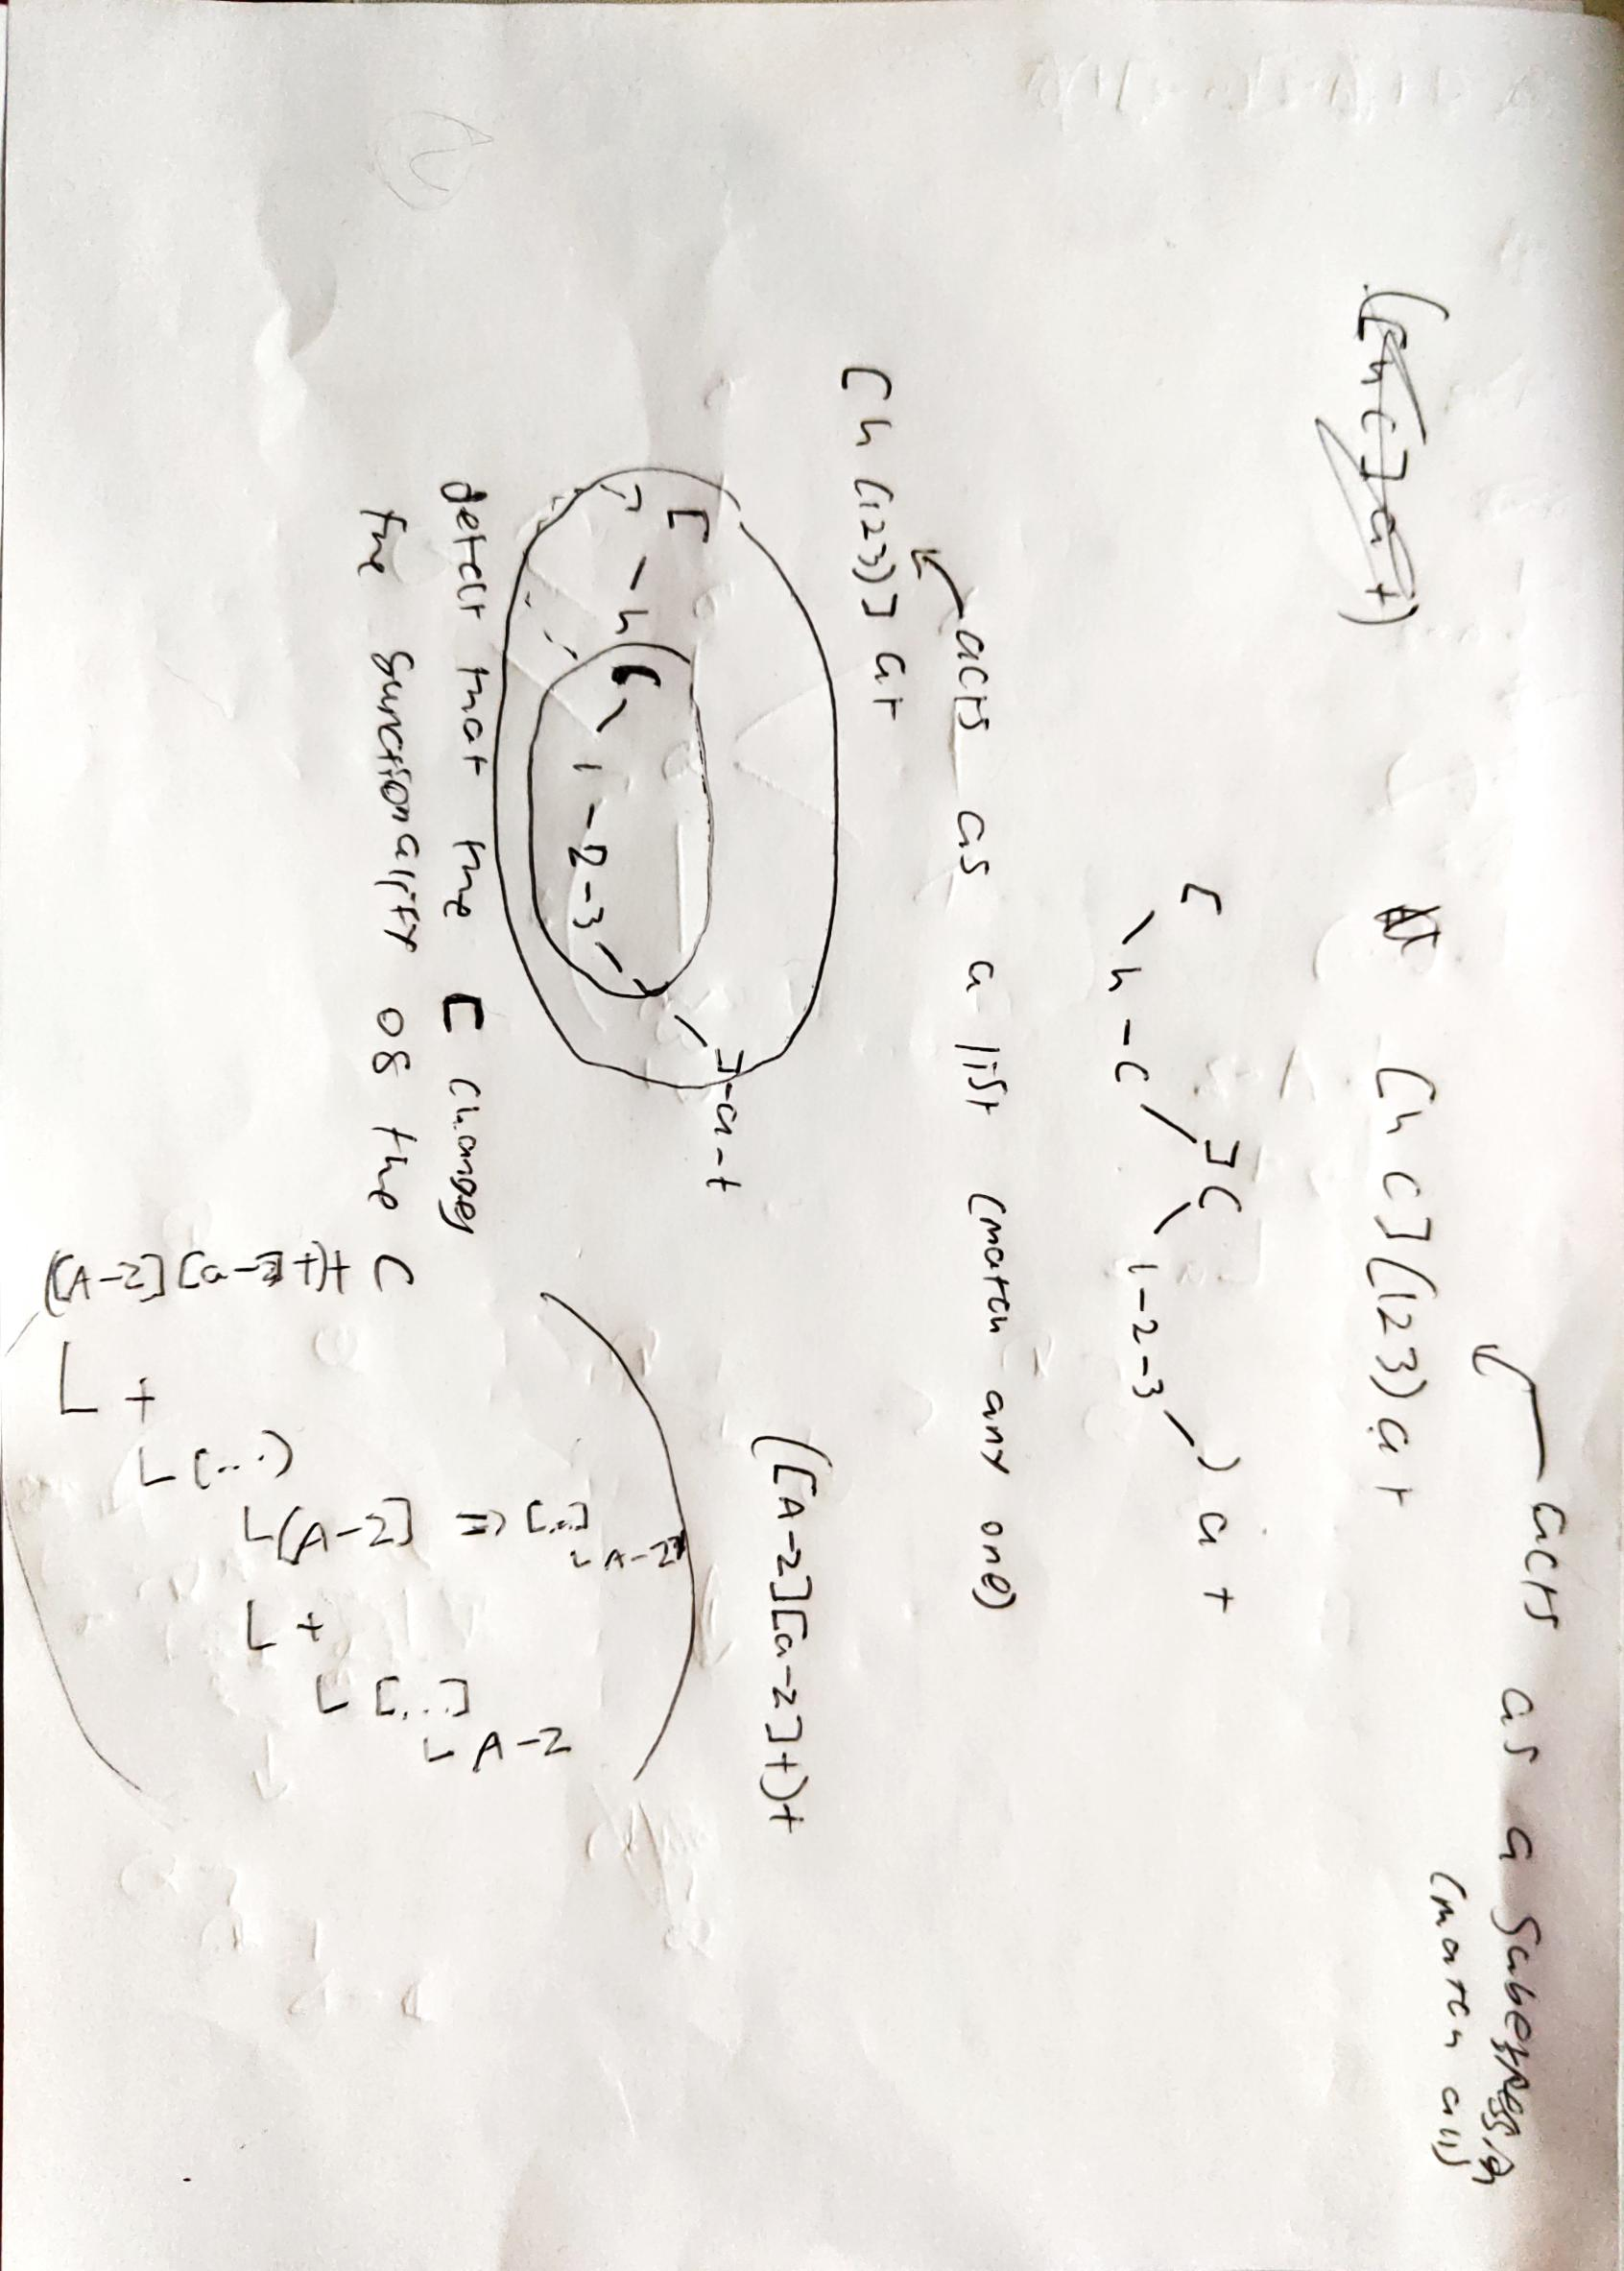
\includegraphics[angle=90,width=0.5\textwidth]{Figures/TokenBreakdown.jpg}
\end{wrapfigure}
One of the major goals of this project was to create a module for the program that would correct the naming of objects, members and variables to match a user-defined style. Regular expressions (regex) are a very powerful algorithm that allows for checking if an input string matches a pattern using a specific syntax. While there are many regex tools available, either through third-party packages or built-in to the programming language, the majority of them are only capable of matching to a string and performing simple replacements on matches within a string. However, converting an input to conform to an output style is a much more complex task as the algorithm needs to be run "in reverse", though it is not as simple as just reversing the regex pattern. With this in mind a new type of regex engine had to be created from scratch to suit the needs of this task.
To start out, the existing syntax for regex was noted, specifically the syntax from the IEEE POSIX standard \citep*{enwiki:1218131380} was investigated.
Theoretical prototypes were created on paper to show how the regex pattern could be deconstructed and reconstructed (see Figure \ref{fig:TokenBreakdown}).
From this syntax, a simplified set was created that would be used for the new regex engine (see Table \ref{tab:SimplifiedRegexSyntax}). This simplified expression set was picked to be simple to implement and easy to read. An advanced language set is not nessecaraly needed either for matching single strings on object names, however there are cases where it could be useful.\\
\begin{table}[h!]
    \centering
    \label{tab:SimplifiedRegexSyntax}
    \begin{tabular}{|p{2cm}|p{3cm}|p{8cm}|}
        \hline
        \multicolumn{3}{|c|}{Simplified Regular Expression Syntax} \\
        \hline
        Symbol&Description&Example\\
        \hline
        \multicolumn{3}{|l|}{Quantifiers}\\
        \hline
        ?&Zero or one&ab?c matches ac and abc\\
        \textasteriskcentered&Zero or more&ab*c matches ac, abc, abbc, abbbc, etc.\\
        +&One or more&ab+c matches abc, abbc, abbbc, etc.\\
        \{\}&Exact number&ab\{2\}c matches abbc\\
        \{n,m\}&Range&ab\{2,4\}c matches abbc, abbbc, abbbbc\\
        \hline
        \multicolumn{3}{|l|}{Group Constructs}\\
        \hline
        ()&Group&ab(cd) matches abcd\\
        \hline
        \multicolumn{3}{|l|}{Meta sequence}\\
        \hline
        \textbackslash s&Whitespace&\\
        \textbackslash S&Non-whitespace&\\
        \textbackslash d&Digit&Matches 0 through to 9\\
        \textbackslash D&Non-digit&\\
        \textbackslash w&Word&Matches letters A to Z case insensitive\\
        \textbackslash W&Non-word&\\
        \hline
        \multicolumn{3}{|l|}{Character Range}\\
        \hline
        []&Character range&[a-c] matches a, b, or c\\
        % []&Negated character range&[\textasciicircum a-c] matches any character except a, b, or c\\
        \string^ &Negated character range&[\string^ a-c] matches any character except a, b, or c\\
        \hline
        \multicolumn{3}{|l|}{Atom}\\
        \hline
        .&Any character&A matches the capital letter A\\
        \hline
    \end{tabular}
\end{table}

% The simplified regex engine would also have limitations when matching certain tokens\dots
